%Here should be an overview of statistical methods used: like bayes factor, ttest, 
\chapter*{Appendix A}
\section*{Statistical Analysis}
\paragraph{T-test}
The t-test or student's t-test is applied to data that is believed to be normally distributed. It is used to determine if two data samples have significantly different means (two-sampled t-test). T-test can be either paired or unpaired. Paired t-test are applied to data sets gained from the same group (e.g. testing the data of the same participant against different conditions,), Unpaired t-test are used when two different groups are tested against each other (e.g. control group against experimental group). 
\paragraph{Cohen's D}
Cohen's d is a measure if the effect size and is based on the differences of the mean. It is calculated by the difference of the means of the two samples, which is then diving by the standard deviation of the data. 
\begin{equation}
    d = \frac{m_1 - m_2}{\sigma}
\end{equation}
As the t-test, Cohen's d can be applied to paired or unpaired tests, while we use the paired test. 
Commonly a results of 0.2 is said to be a small effect size, while larger numbers like 0.8 are interpreted as large effect sizes. 
\paragraph{Bayes Factor}
The Bayes Factor is an alternative to statistical hypothesis testing like the t-test. It is aimed to show the support of one model over another model (or of one hypothesis over another hypothesis), regardless if either of them is true. 
It is calculated dividing the likelihood given the data by model one (or the alternative hypothesis) by the likelihood given the data by model zero (or Null hypothesis). 
Usually, a Bayes Factor over 100 is extreme high evidence for the alternative hypothesis or model, whereas below 10 it is rather moderate, while below 0 it favours the other hypothesis. 
\paragraph{Spearman's $\rho$}
Spearman's $\rho$ is a non-parametric rank test used to see if two samples are correlated. Unlike Pearsons correlation rank test, it can also asses not linear relationships. It is, however, based on Pearsons 
\subsection*{Statistical Tests on the Parameters}
\paragraph{Wilcox signed rank test}

\chapter*{Appendix B}
\section*{Model analysis}
\paragraph{Crossvalidation}
\paragraph{Simulation}
\paragraph{Parameter Recovery}

\chapter*{Appendix C}
\section*{Modelling Results}
\subsection*{Model Comparison}
\begin{figure}
    \centering
    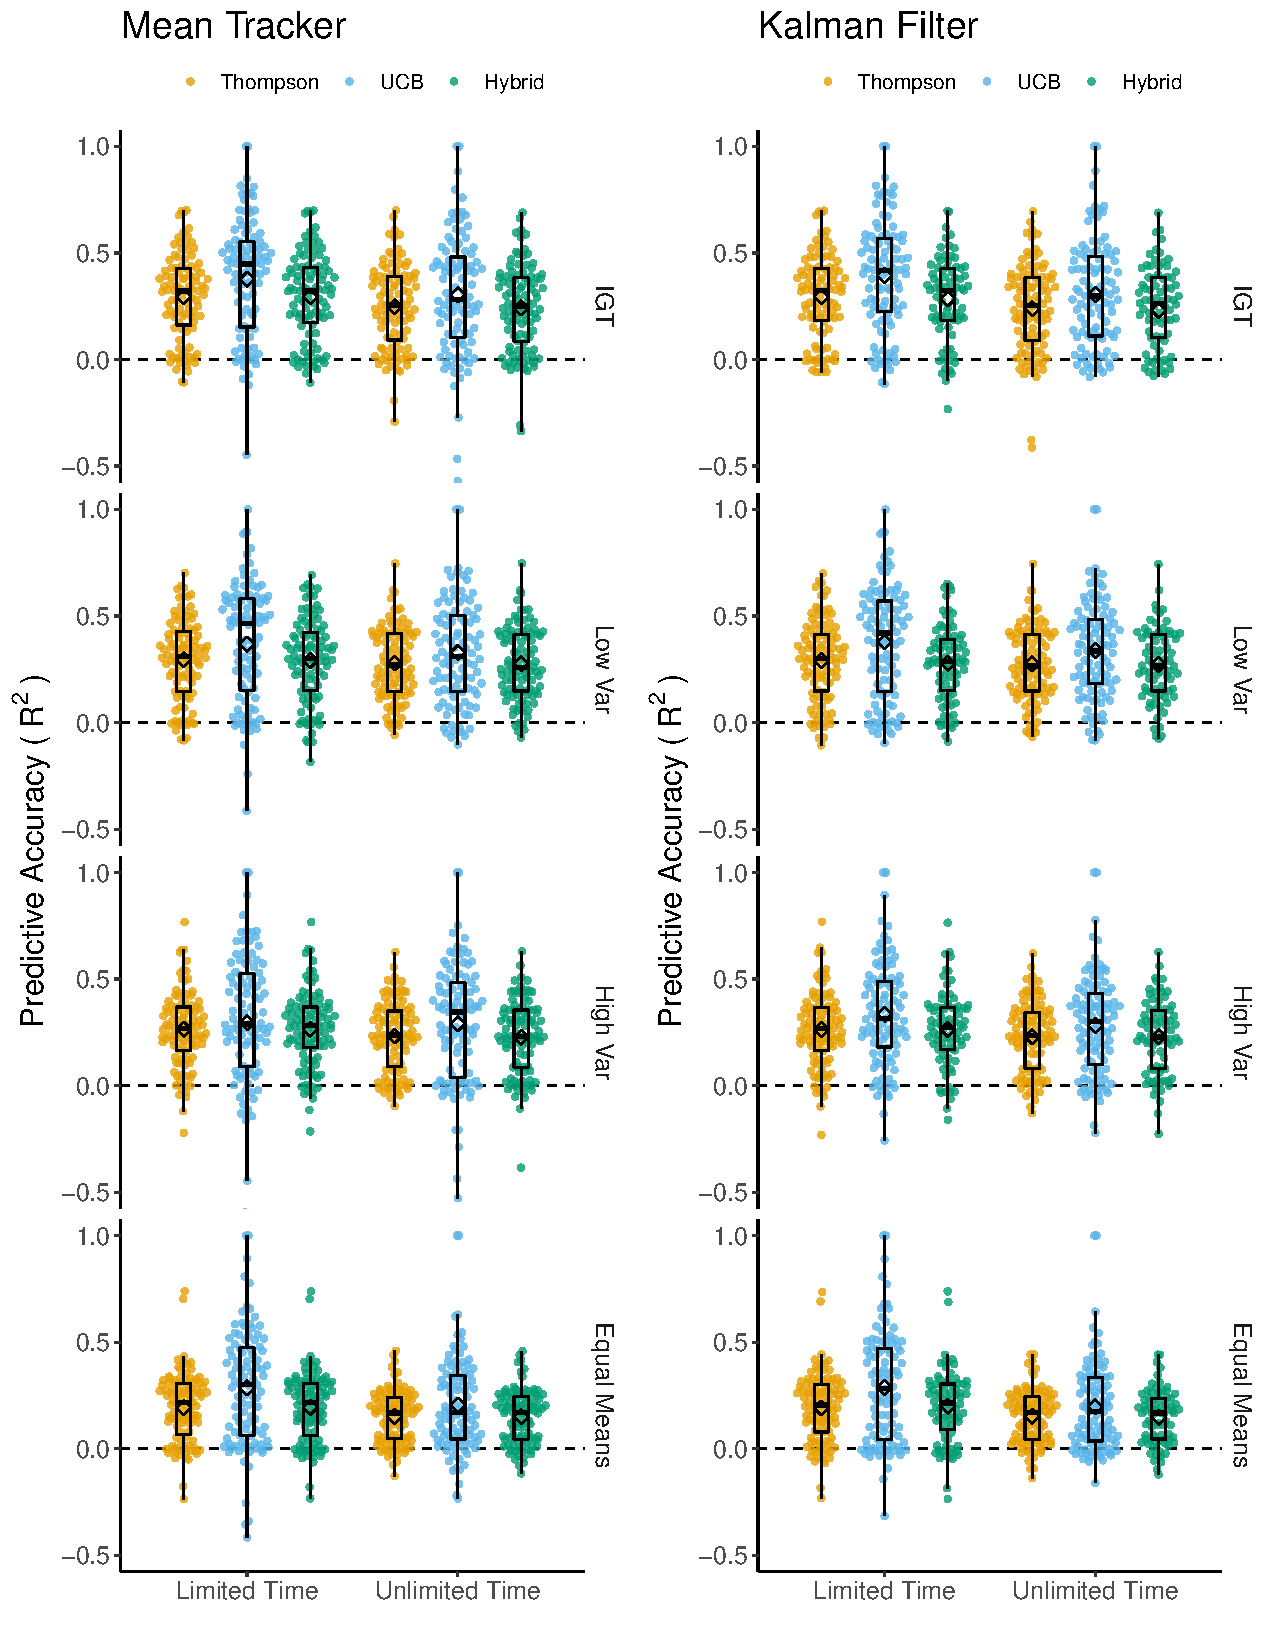
\includegraphics[1\textwidth]{Plots/KF&BMT_Accuracy.pdf}
    \caption{The Accuracy of the KF and the BMT over all participants for all conditions}
    \label{fig:AllR2}
\end{figure}

\begin{table}[h!]
\begin{adjustwidth}{-2.5cm}{}
\vspace{-2mm}
\caption{Best Fitted Model for all Conditions and PayoffCondition Combinations} 
\label{tab:All_Fitted} 
\begin{tabular*}{1.5\textwidth}{@{}l@{}|l@{}|c@{}|c@{}|c@{}|c@{}|c@{}|c@{}}
\toprule
Payoff Condition&Time Conditions & KF-UCB &KF-Thompson& KF-Hybrid & BMT-UCB & BMT-Thompson & BMT-Hybrid  \\ \midrule
All&All&$290$ &$39$ &$27$ &$345$ & $54$ & $37$\\
All&Unlimited Time &$140$ &$19$ &$13$ &$172$ & $32$ &$20$\\
All&Limited Time &$150$& $20$&$14$&$173$&$22$&$17$\\
IGT&All & $79$  & $8 $& $7$ & $86$ & $14$ & $4$     \\
IGT&Unlimited Time  & $34$ & $5$ & $5$ & $44$ &$8$ & $3$ \\
IGT&Limited Time  & $45$ & $3$ & $2$ & $42$ &$6$ & $1$   \\
Low Var&All & $76$  & $11 $& $4$ & $80$ & $8$ & $19$     \\
Low Var&Unlimited Time  & $40$ & $5$ & $2$ & $37$ &$4$ & $11$ \\
Low Var&Limited Time  & $36$ & $6$ & $2$ & $43$ &$4$ & $8$   \\
High Var&All & $80$  & $9$ & $3$ & $84$ & $17$ & $5$     \\
High Var&Unlimited Time  & $41$ & $5$ & $1$ & $42$ &$10$ & $0$  \\
High Var&Limited Time  & $39$ & $5$ & $1$ & $41$ &$7$ & $5$   \\
Equal Means&All & $55$  & $11$ & $12$ & $96$ & $15$ & $9$     \\
Equal Means&Unlimited Time  & $25$ & $4$ & $5$ & $49$ &$10$ & $6$  \\
Equal Means&Limited Time  & $30$ & $7$ & $7$ & $47$ &$5$ & $3$   \\
\bottomrule
\end{tabular*}
\vspace{5mm}
\end{adjustwidth}
\end{table}

\subsection*{Paramater Estimates}

\begin{table}[h!]
\vspace{-2mm}
\caption{Median Parameters for all combination over best fitted models} 
\label{tab:AllbestParam} 
\begin{tabular*}{\textwidth}{@{}ll@{\extracolsep{\fill}}cccc@{}}
\toprule
Payoff Condition&Time Conditions & $\tau$ &$\beta$  & $\theta_\epsilon^2$&$\omega$  \\ \midrule
All&All&$30.5$ &$3.03$ &$3.8$ & $84.4$ \\
All&Unlimited Time &$43.7$ &$8$ &$2.1$ &$114.8$ \\
All&Limited Time &$21.2$& $2.2$&$5.8$&$57.8$\\
IGT&All & $15.9$  & $0.8 $& $5.7$ & $30.03$     \\
IGT&Unlimited Time  & $16.2$ & $0.5$ & $4.5$ & $21.1$\\
IGT&Limited Time  & $12.5$ & $1.5$ & $7.2$ & $36.5$  \\
Low Var&All & $21.9$  & $10.1 $& $1.9$ & $58.9$     \\
Low Var&Unlimited Time  & $26$ & $16.7$ & $1.2$ & $60$  \\
Low Var&Limited Time  & $21.9$ & $3.9$ & $3$ & $51.6$   \\
High Var&All & $22.9$  & $6.2$ & $2.4$ & $65.9$    \\
High Var&Unlimited Time  & $27.4$ & $20$ & $1.5$ & $71.1$  \\
High Var&Limited Time  & $11.3$ & $2.9$ & $5.7$ & $44.3$   \\
Equal Means&All & $113.4$  & $0.2$ & $4.8$ & $292$      \\
Equal Means&Unlimited Time  & $142$ & $1$ & $3.2$ & $302.3$   \\
Equal Means&Limited Time  & $93.8$ & $0.01$ & $7.8$ & $292$    \\
\bottomrule
\end{tabular*}
\vspace{5mm}
\end{table}